\documentclass[aspectratio=169,11pt,red]{beamer}
\usepackage{beamerthemeshadow} %tema
\beamertemplateshadingbackground{black!5}{white!15}  %cores de fundo
\beamertemplatenavigationsymbolsempty %retirar a barra de navegação

\usepackage[utf8]{inputenc}
\usepackage[T1]{fontenc}
\usepackage[brazil]{babel}
\usepackage[portuguese, ruled, linesnumbered]{algorithm2e}
\usepackage{multicol}
\usepackage{graphicx}
\graphicspath{ {imagens/} }

\newcommand{\disp}{\displaystyle}

\author[\sc{GREGORIIS, G.}]{Aluna: Giordanna De Gregoriis\\Orientadora: Cristina Lúcia Dias Vaz\\Co-Orientador: Dionne Cavalcante Monteiro}
\institute[\sc{UFPA}]{Universidade Federal do Pará\\Instituto de Ciências Exatas e Naturais\\Faculdade de Computação\\Bacharelado em Ciência da Computação}
\date{\today}

\title{Trabalho Parcial Sobre o Estudo Desenvolvido}
\begin{document}

\begin{frame}
\titlepage
\end{frame}

\begin{frame}
\begin{multicols}{2}
{\tableofcontents}
\end{multicols}
\end{frame}

\section{Introdução}
\begin{frame}
\frametitle{Introdução}

$\bullet$ Este seminário tem como objetivo mostrar os resultados do que já foi obtido até o momento;
\medskip
\pause

$\bullet$ Na primeira seção é mostrado os resultados do estudo feito em torno do artigo {\it ``The Art of Random Fractals''}, escrito por Douglas Dunham e John Shier, onde é explicado o funcionamento e a matemática do algoritmo de demonstração, com as devidas considerações finais e o resumo dos resultados obtidos;
\medskip
\pause

$\bullet$ Na segunda seção tem-se o início de um estudo a respeito do fractal Apolloniano, onde para melhor compreensão foi feita a sua implementação.
\medskip

\end{frame}

\section{Estudo do Artigo ``The Art Of Random Fractals''}
\subsection{Estudo do Artigo ``The Art Of Random Fractals''}
\begin{frame}
\frametitle{Estudo do Artigo ``The Art Of Random Fractals''}

$\bullet$ O algoritmo criado por John Shier possui uma base matemática que permite preencher uma região espacial com uma sequência finita de formas (ou ``estampas'', como ele descreve) colocadas aleatoriamente e cada vez menores;
\medskip
\pause

$\bullet$ Este algoritmo pode ser usado para produzir uma variedade de padrões que são esteticamente agradáveis, que pela sua aparente autossimilaridade são chamados de padrões fractais.
\medskip

\end{frame}

\subsubsection{Início}
\begin{frame}
\frametitle{Início}

Inicialmente desejava-se preencher área $A$ com estampas em posições aleatórias, progressivamente menores, sem que estas tenham intersecção entre si. Foi descoberto através de testes que isso pode ser alcançado se for obedecido uma regra de potência inversa;
\medskip
\pause

Para $i=0, 1, 2, ...$ a área da estampa de ordem $i$, $A_{i}$ pode ser definido por:
\medskip

\begin{equation}
A_{i} = \dfrac{A}{\zeta(c,N)(N+i)^c}
\end{equation}
\medskip

Onde $c>1$, $c_{max}\approx1.48$ e $N>1$ são parâmetros, e $\zeta(c,N)$ é a função zeta de Hurwitz: $$\zeta(c,N)=\sum\limits_{k=0}^\infty\dfrac{1}{(N+k)^c}$$
\medskip

\end{frame}

\begin{frame}
\frametitle{Função Zeta de Hurtwitz}

A função zeta de Hurwitz implementada no algoritmo original é feita apenas no domínio dos números reais, feita com somatórios aproximados. Esta função aproximada é dada por:
\medskip

\begin{equation}
\zeta(c,N) = (\sum\limits_{i=N}^{100000} i^{-c})+(\dfrac{1}{c-1} \times N^{1-c})
\end{equation}

\end{frame}

\begin{frame}
\frametitle{Função Zeta de Hurtwitz}

No algoritmo de demonstração o $c$ é um valor encontrado aleatoriamente entre $1$ e $1.48$ e $N=2$.
\medskip

O número retornado por esta função será utilizado para determinar a porcentagem da área $A$ que será preenchida por $A_{0}$. \pause \textbf{Exemplo:}
\medskip

\begin{equation}
\zeta(1.263,2) = (\sum\limits_{i=2}^{100000} i^{-1.263})+(\dfrac{1}{1.263-1} \times 2^{1-1.263})
\end{equation}
$$\approx 3.23 + 0.19 \approx 3.42$$

\end{frame}

\begin{frame}
\frametitle{Início}

Com $c=1.263$ e $N=2$, o valor obtido de $\zeta(1.263,2)$ foi aproximadamente $3.42$. O algoritmo então procede calculando a razão através de: 
\medskip

\begin{equation}
Raz\tilde{a}o=\dfrac{1}{\zeta(1.263,2)}=\dfrac{1}{3.42}\approx0.29
\end{equation}
\medskip

Então a área $A_{0}$ da primeira forma a ser posicionada no plano deverá preencher aproximadamente $29\%$ da área original.
\medskip

\end{frame}

\begin{frame}
\frametitle{Início}

Na demonstração original deseja-se preencher o plano com círculos. Para isso utiliza-se a razão para descobrir qual será o raio do primeiro círculo que terá área $A_{0}$, dada por:
\medskip

\begin{equation}
Raio_{A_{0}}= (\sqrt{A_{total}} \times \sqrt{\dfrac{Raz\tilde{a}o}{\pi}}) \times N^{-\dfrac{c}{2}} 
\end{equation}
\medskip

Onde $N^{-\dfrac{c}{2}}$ serve para reduzir o valor obtido de acordo com a iteração $N$, assim servindo para a parte iterativa do algoritmo também.
\medskip

\end{frame}

\begin{frame}
\frametitle{Início}

Substituindo a fórmula anterior pelos valores do exemplo dado alguns slides atrás e considerando que a nossa área é uma tela de $600 \times 600$ pixels, temos:
\medskip

\begin{equation}
Raio_{A_{0}} = (\sqrt{360000} \times \sqrt{\dfrac{0.29}{\pi}}) \times 2^{-\dfrac{1.263}{2}}
\end{equation}

$$
\approx (600 \times 0.3) \times 2^{-0.6315} \approx 180 \times 0.64 \approx 115.2
$$

\end{frame}

\subsubsection{Iteração}
\begin{frame}
\frametitle{Iteração}

$\bullet$ Quando $i = 0$, a primeira forma com área de $A_{0}$ é colocada aleatóriamente no interior da região $R$ tal que não se sobreponha a fronteira de $R$. Isso normalmente requer várias tentativas em posições aleatórias antes da obtenção de um posicionamento bem sucedido em que a forma é completamente dentro de $R$;
\medskip
\pause

$\bullet$ Quando $i > 0$, para cada $i = 1, 2, ..., n$ coloca-se de forma iterativa aleatoriamente uma cópia da estampa com área $A_{i}$ dentro de $R$ e de modo que não intersecte com qualquer cópia anteriormente colocada. Em seguida, passamos a colocar a próxima estampa, com área de $A_{i + 1}$, ou parar o algoritmo se foi colocado a $n$-ésima forma ou atingiu uma outra condição de parada.
\medskip

\end{frame}

\begin{frame}
\frametitle{Iteração}

O raio da forma $A_{i}$ $i$ para $i > 0$ é determinado por:
\medskip

\begin{equation}
Raio_{A_{i}}= Raio_{A_{0}} \times i^{-\dfrac{c}{2}} 
\end{equation}
\medskip

Onde $Raio_{A_{0}}$ é o raio da primeira forma inserida no plano.
\medskip

\end{frame}

\begin{frame}
\frametitle{Iteração}

$\bullet$ Após determinar uma posição aleatória no plano, verifica-se caso a forma $A_{i}$ não intersecta com nenhuma outra já posicionada. Este teste depende de cada forma, devendo ser implementado de acordo com suas características. Caso seja desejável inserir formas diferentes no mesmo plano, o teste deve ser abstraído para aceitar qualquer entrada e produzir uma resposta correta.
\medskip
\pause

$\bullet$ Neste algoritmo demonstratívo, o teste é feito apenas para círculos. Além disso ele verifica se a distância entre os círculos é maior que a soma de seus raios, evitando assim que os círculos sejam posicionados muito próximo entre si e tornando a imagem mais esteticamente agradável.
\medskip

\end{frame}

\begin{frame}
\frametitle{Iteração}

\begin{algorithm}[H]
   \SetAlgoLined
   \Entrada{$x_{1}, y_{1}, raio_{1}, x_{2}, y_{2}, raio_{2}$} 
   \Saida{$true$ se não tem intersecção e $false$ caso contrário}
   \Inicio{
    \Se{$\vert x_{1} - x_{2}\vert < (raio_{1} + raio_{2})$}{
        \Se{$\vert y_{1} - y_{2}\vert < (raio_{1} + raio_{2})$}{
            \Se{$\sqrt{(x_{1}-x_{2})^2 + (y_{1}-y_{2})^2} >= (raio_{1} + raio_{2})$}{
                \Retorna{true}
            }
        }
    }
   }
   \Retorna{false}
   \label{alg1}
   \caption{\textsc{Teste de intersecção dos círculos}}
 \end{algorithm}

\end{frame}

\subsubsection{Finalização}
\begin{frame}
\frametitle{Finalização}
Terminado a iteração temos uma figura que se assemelha a um fractal geométrico aleatório onde nenhuma das estampas se tocam, e a área não preenchida ou carpete é um conjunto conectado contínuo (isso se forem estampas sem oco).
\end{frame}

\begin{frame}
\frametitle{Finalização}

\begin{figure}[h]
\caption{Exemplo de uma execução, com $c=1,3$}
\centering
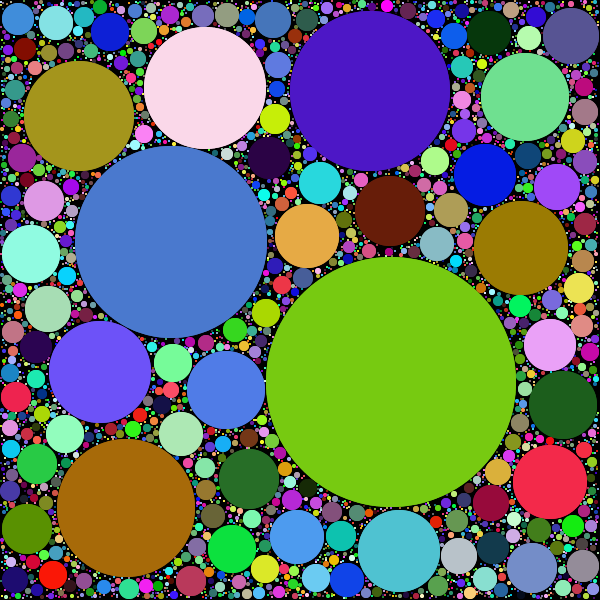
\includegraphics[width=\textwidth,height=0.7\textheight,keepaspectratio]{exemplo1}
\end{figure}

\end{frame}

\subsection{Testes e Resultados}
\begin{frame}
\frametitle{Testes e Resultados}
Vários testes foram realizados para entender melhor a relação entre os diversos parâmetros presentes no algoritmo.
\medskip

Foi desenvolvido um aplicativo em Java onde se insere um valor $c$, sendo seus limites $1,01 \leqslant c \leqslant 1,48$. Depois de inserido o valor, inicia o processo de geração da imagem em uma tela de $600 \times 600$ pixels e $N=2$.

\end{frame}

\subsubsection{Círculo}

\begin{frame}
\frametitle{Círculo}
\begin{columns}[T]
\begin{column}{.5\textwidth}
\begin{block}{\centering Dados}
$c=1,48$
\smallskip

$\zeta(c,N)=1,694351369474375$
\smallskip

Razão $=0,5901963536112477$
\smallskip

Raio $=155,70852052297627$
\smallskip

$A_{preenchida} \approx 93\%$
\smallskip

Nº de iterações $=400000$
\smallskip

Nº de formas $=2434$
\smallskip

tempo de execução $= 0,274$ segundos.
\smallskip
\end{block}
\end{column}

\begin{column}{.5\textwidth}
\begin{block}{\centering Resultado}
\centering

\includegraphics[width=0.7\textwidth]{exemplo2}
\end{block}
\end{column}
\end{columns}
\end{frame}

\begin{frame}
\frametitle{Círculo}

\begin{columns}[T]
\begin{column}{.5\textwidth}
\begin{block}{\centering Dados}
$c=1,24$
\smallskip

$\zeta(c,N)=3,7610743206468737$
\smallskip

Razão $=0,26588147820168795$
\smallskip

Raio $=113,57474202778332$
\smallskip

$A_{preenchida} \approx 78\%$
\smallskip

Nº de iterações $=374108$
\smallskip

Nº de formas $=90001$
\smallskip

tempo de execução $= 47,798$ segundos.
\smallskip
\end{block}
\end{column}

\begin{column}{.5\textwidth}
\begin{block}{\centering Resultado}
\centering
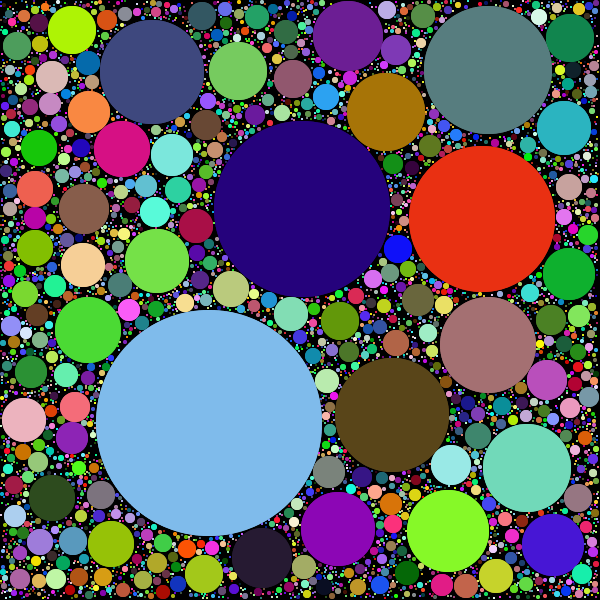
\includegraphics[width=0.7\textwidth]{exemplo3}
\end{block}
\end{column}
\end{columns}

\end{frame}

\begin{frame}
\frametitle{Círculo}

\begin{columns}[T]
\begin{column}{.5\textwidth}
\begin{block}{\centering Dados}
$c=1,01$
\smallskip
$\zeta(c,N)=99,5779388822347$
\smallskip

Razão $=0,010042385002391388$
\smallskip

Raio $=23,90422124959249$
\smallskip

$A_{preenchida} \approx 5\%$
\smallskip

Nº de iterações $=94017$
\smallskip

Nº de formas $=90001$
\smallskip

tempo de execução $=61,888$ segundos.
\smallskip
\end{block}
\end{column}

\begin{column}{.5\textwidth}
\begin{block}{\centering Resultado}
\centering

\includegraphics[width=0.7\textwidth]{exemplo4}
\end{block}
\end{column}
\end{columns}
\end{frame}

\subsubsection{Quadrado}
\begin{frame}
\frametitle{Quadrado}
\begin{columns}[T]
\begin{column}{.5\textwidth}
\begin{block}{\centering Dados}
$c=1,48$
\smallskip

$\zeta(c,N)=1,694351369474375$
\smallskip

Razão $=0,5901963536112477$
\smallskip

Raio $=137,99308340987494$
\smallskip

$A_{preenchida} \approx 86\%$
\smallskip

Nº de iterações $=406508$
\smallskip

Nº de formas $=120$
\smallskip

tempo de execução $= 0,271$ segundos.
\smallskip
\end{block}
\end{column}

\begin{column}{.5\textwidth}
\begin{block}{\centering Resultado}
\centering
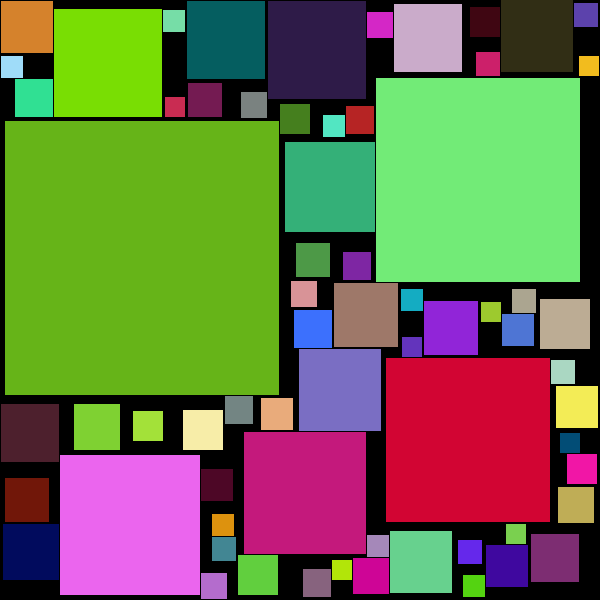
\includegraphics[width=0.7\textwidth]{exemplo5}
\end{block}
\end{column}
\end{columns}
\end{frame}

\begin{frame}
\frametitle{Quadrado}
\begin{columns}[T]
\begin{column}{.5\textwidth}
\begin{block}{\centering Dados}
$c=1,24$
\smallskip

$\zeta(c,N)=3,7610743206468737$
\smallskip

Razão $=0,26588147820168795$
\smallskip

Raio $=100,65299443637255$
\smallskip

$A_{preenchida} \approx 77\%$
\smallskip

Nº de iterações $=400038$
\smallskip

Nº de formas $=33432$
\smallskip

tempo de execução $= 12,492$ segundos.
\smallskip
\end{block}
\end{column}

\begin{column}{.5\textwidth}
\begin{block}{\centering Resultado}
\centering
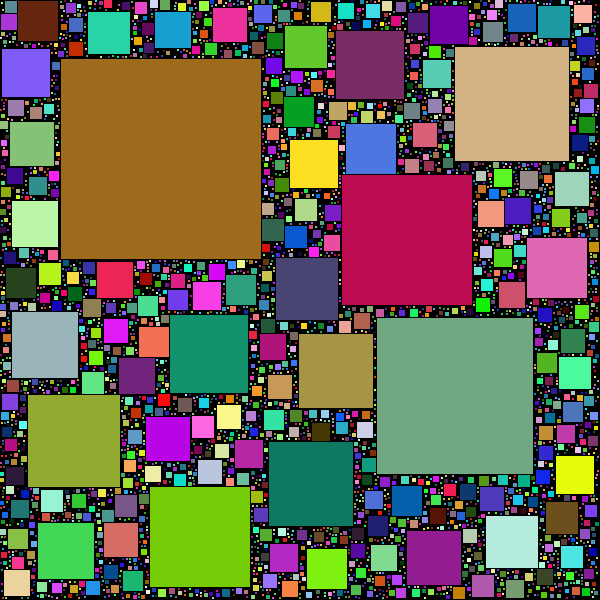
\includegraphics[width=0.7\textwidth]{exemplo6}
\end{block}
\end{column}
\end{columns}
\end{frame}

\begin{frame}
\frametitle{Quadrado}
\begin{columns}[T]
\begin{column}{.5\textwidth}
\begin{block}{\centering Dados}
$c=1,01$
\smallskip
$\zeta(c,N)=99,5779388822347$
\smallskip

Razão $=0,010042385002391388$
\smallskip

Raio $=21,184564503368836$
\smallskip

$A_{preenchida} \approx 4\%$
\smallskip

Nº de iterações $=111583$
\smallskip

Nº de formas $=90001$
\smallskip

tempo de execução $=256,638$ segundos.
\smallskip
\end{block}
\end{column}

\begin{column}{.5\textwidth}
\begin{block}{\centering Resultado}
\centering
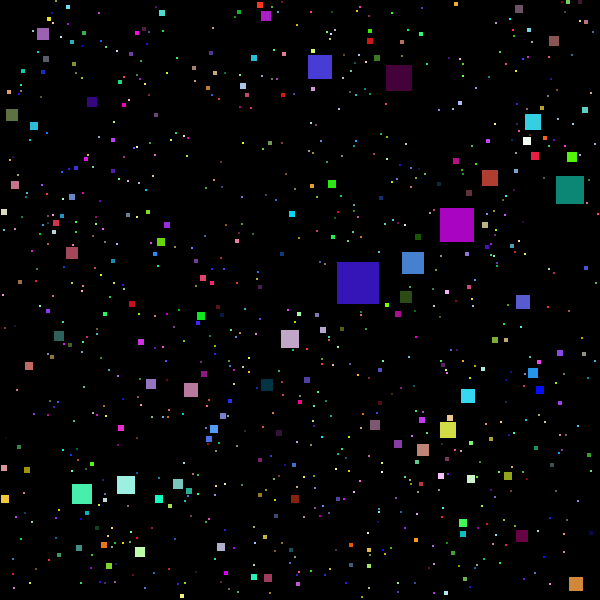
\includegraphics[width=0.7\textwidth]{exemplo7}
\end{block}
\end{column}
\end{columns}
\end{frame}

\subsection{Considerações Finais desta Seção}
\begin{frame}
\frametitle{Considerações Finais desta Seção}
$\bullet$ Os métodos apresentados criam imagens artísticas, que são uma mistura de geometria e aleatoriedade;
\medskip

$\bullet$ Quanto maior o fator $c$, maior o tamanho do raio da primeira forma a ser colocada no quadro, maior a porcentagem do preenchimento da área, menor será a quantidade de formas, menor o tempo de execução e mais rapidamente as formas vão diminuindo de tamanho;
\medskip

$\bullet$ Pode-se observar que a colocação de novas formas geralmente é interrompida quando o raio da próxima forma é inferior a $3,5\%$ do raio da maior forma (a primeira).
\end{frame}

\section{Utilização e Implementação do Fractal Apolloniano}
\subsection{Utilização e Implementação do Fractal Apolloniano}
\begin{frame}
\frametitle{Utilização e Implementação do Fractal Apolloniano (em andamento)}

$\bullet$ O fractal criado pelo matemático grego Apollonius of Perga baseia-se em gerar ``trincas'' de círculos, onde cada um é tangente aos outros dois;
\medskip
\pause

$\bullet$ Pode ser usado para preencher com mais eficácia uma determinada área, além de produzir resultados esteticamente agradáveis.
\medskip

\end{frame}

\subsection{Algoritmo}
\begin{frame}
\frametitle{Algoritmo}
Para programar este fractal foi utilizado o algoritmo de Soddy, no qual inicia-se com 3 círculos de curvaturas $k (k_{ia}, k_{ib}, k_{ic})$.
\medskip

O algoritmo utiliza os círculos definidos pelos centros $c_{n}$ e curvaturas $k_{n}$, e também o teorema dos círculos de Descartes para encontrar a curvatura do próximo círculo $k_{4}$.
\medskip

\begin{equation}
k_{4} = k_{1} + k_{2} + k_{3} \pm 2 \sqrt{k_{1}k_{2} + k_{2}k_{3} + k_{3}k_{1}}
\end{equation}
\end{frame}

\begin{frame}
\frametitle{Algoritmo}
Utiliza-se do teorema de círculos complexos de Descartes para encontrar o centro do círculo $c_{4}$.
\medskip

\begin{equation}
c_{4} = \dfrac{c_{1}k_{1} + c_{2}k_{2} + c_{3}k_{3} \pm 2 \sqrt{k_{1}k_{2}c_{1}c_{2} + k_{2}k_{3}c_{2}c_{3} + k_{3}k_{1}c_{3}c_{1}}}{k_{4}}
\end{equation}
\end{frame}

\begin{frame}
\frametitle{Algoritmo}
Encontra-se um raio do primeiro círculo a ser colocado. Isto pode ser aleatório ou pré-definido. Neste programa estes valores são computados por porcentagens, ou seja, valores de $0,5 < raio_{0} < 1$. Assim o primeiro círculo deve ser no mínimo um pouco maior que a metade do lado do quadrado do nosso quadro.
\medskip

Acha-se o valor que será usado para encontrar as posições X e Y do centro do primeiro círculo.
\medskip

$$valor = \dfrac{\pi}{2}-arcseno(aleatorio \times (1-raio_{0})/raio_{0})$$
$$X_{primeiro} = raio_{0} \times cos(valor)$$
$$Y_{primeiro} = raio_{0} \times sen(valor)$$
\end{frame}

\begin{frame}
\frametitle{Algoritmo}
Número de círculos novos no estágio $n = 2 \times 3^{n}$
\medskip

Número total de círculos depois de $n$ estágios $= 2 \times 3^{n+1}$
\end{frame}

\begin{frame}
\frametitle{Algoritmo}
Terminado a iteração temos um fractal Apolloniano composto por círculos que se tangenciam levemente.
\end{frame}

\begin{frame}
\frametitle{Algoritmo}

\begin{figure}[h]
\caption{Exemplo de uma execução, com $c=1,3$}
\centering
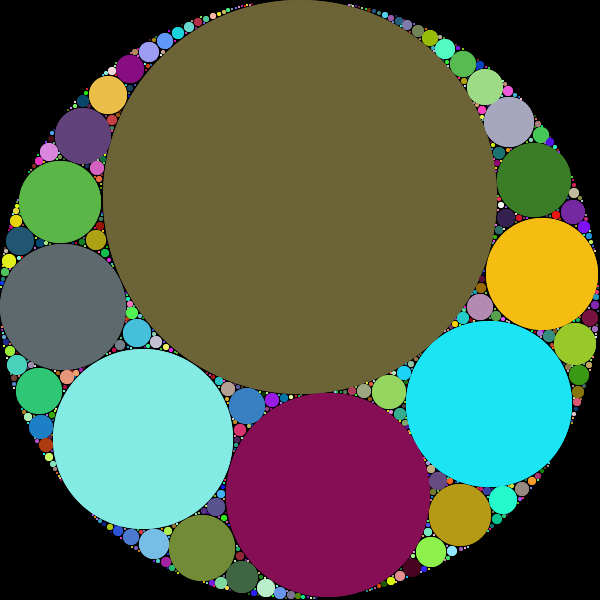
\includegraphics[width=\textwidth,height=0.7\textheight,keepaspectratio]{apolloniano1}
\end{figure}

\end{frame}

\subsection{Testes e Resultados}
\begin{frame}
\frametitle{Testes e Resultados}
Alguns testes foram realizados para verificar se era possível reaproveitar a razão do raio gerada a partir da função Zeta de Hurtwitz na geração do primeiro círculo do fractal.
\medskip

Foi desenvolvido um aplicativo em Java onde se insere um valor $c$, sendo seus limites $1,01 \leqslant c \leqslant 1,48$. Depois de inserido o valor, inicia o processo de geração da imagem em uma tela de $600 \times 600$ pixels.

\end{frame}

\begin{frame}
\frametitle{Testes e Resultados}
\begin{columns}[T]
\begin{column}{.5\textwidth}
\begin{block}{\centering Dados}
$c=1,48$
\smallskip

$\zeta(c,N)=1,694351369474375$
\smallskip

Razão $=0,5901963536112477$
\smallskip

$A_{preenchida} \approx 96\%$
\smallskip

Nº de formas $=3325$
\smallskip

tempo de execução $= 0,187$ segundos.
\smallskip
\end{block}
\end{column}

\begin{column}{.5\textwidth}
\begin{block}{\centering Resultado}
\centering
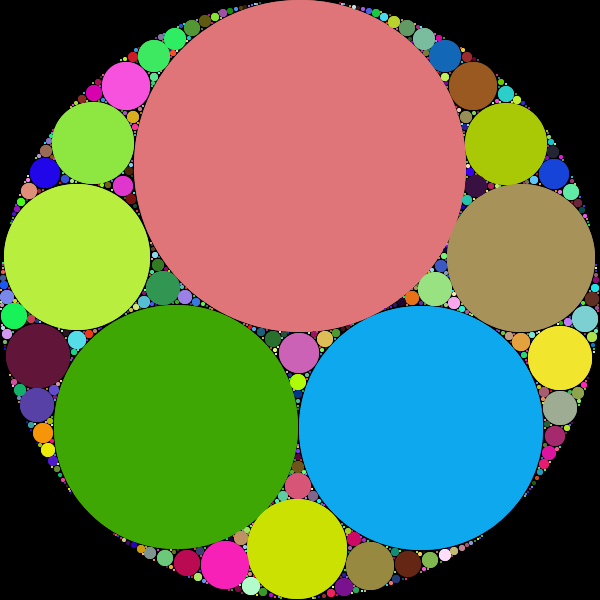
\includegraphics[width=0.7\textwidth]{apolloniano2}
\end{block}
\end{column}
\end{columns}
\end{frame}

\begin{frame}
\frametitle{Testes e Resultados}
\begin{columns}[T]
\begin{column}{.5\textwidth}
\begin{block}{\centering Dados}
$c=1,24$
\smallskip

$\zeta(c,N)=3,7610743206468737$
\smallskip

Razão $=0,26588147820168795$
\smallskip

$A_{preenchida} \approx 95\%$
\smallskip

Nº de formas $=3140$
\smallskip

tempo de execução $= 0,19$ segundos.
\smallskip
\end{block}
\end{column}

\begin{column}{.5\textwidth}
\begin{block}{\centering Resultado}
\centering
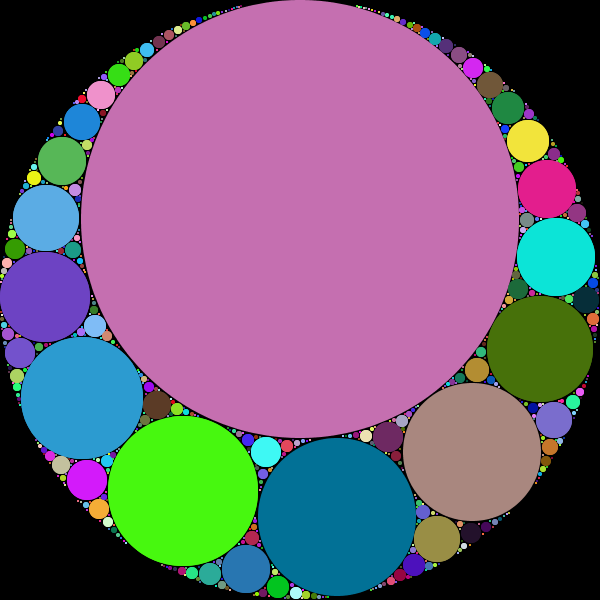
\includegraphics[width=0.7\textwidth]{apolloniano3}
\end{block}
\end{column}
\end{columns}
\end{frame}

\begin{frame}
\frametitle{Testes e Resultados}
\begin{columns}[T]
\begin{column}{.5\textwidth}
\begin{block}{\centering Dados}
$c=1,01$

\smallskip
$\zeta(c,N)=99,5779388822347$
\smallskip

Razão $=0,010042385002391388$
\smallskip

Neste caso foi utilizado: $1-$Razão$=0,989957614997608612$
\smallskip

$A_{preenchida} \approx 98\%$
\smallskip

Nº de formas $=1353$
\smallskip

tempo de execução $=0,74$ segundos.
\smallskip
\end{block}
\end{column}

\begin{column}{.5\textwidth}
\begin{block}{\centering Resultado}
\centering
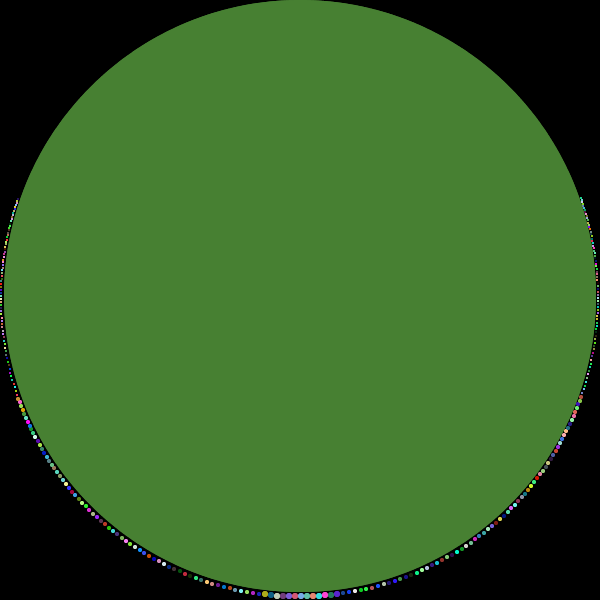
\includegraphics[width=0.7\textwidth]{apolloniano4}
\end{block}
\end{column}
\end{columns}
\end{frame}

\subsection{Considerações Finais desta Seção}
\begin{frame}
\frametitle{Considerações Finais desta Seção}
$\bullet$ O método apresentado cria um fractal que preenche a área desejada com uma boa porcentagem;
\medskip

$\bullet$ O fator $c$ neste caso serviu para obtermos a razão da área, que foi justamente o valor utilizado para definir o tamanho do primeiro círculo da série. Como ele não permite que o primeiro círculo tenha uma razão menor que $0,5$ realiza-se uma ``inversão'' do valor realizando a operação Razão$_{nova} = 1-$Razão$_{antiga}$, assim quanto menor a razão antes de $0,5$, maior será o raio do primeiro círculo;
\medskip

$\bullet$ A sua formação é diferente dos métodos apresentados ateriormente pois neste caso há intersecção entre as formas, porém para resolver esteticamente este problema basta decrementar $0,5$ do raio antes de desenhar as formas no programa.
\end{frame}

\section{Referências}

\begin{frame}
\frametitle{Referências}

Dunham, Douglas, and John Shier. "The Art of Random Fractals." Bridges Seoul,(eds. Gary Greenfield, George Hart, and Reza Sarhangi), Seoul, Korea (2014): 79-86.
\bigskip

Wikibooks, The Free Textbook Project (2013) ``Fractals/Apollonian fractals.'', <https://en.wikibooks.org/wiki/Fractals/Apollonian\_fractals>. Setembro.

\end{frame}

\end{document}

